\newpage
МРНТИ 50.43.15
\hfill {\bfseries \href{https://doi.org/10.58805/kazutb.v.3.24-503}{https://doi.org/10.58805/kazutb.v.3.24-503}}

\sectionwithauthors{М.Г. Жартыбаева, А.Д. Алинова, Ж.О. Оралбекова, Г.А. Тюлепбердинова, Н.М. Жамишева}{ПОСТРОЕНИЕ ТРАЕКТОРИЙ ДЛЯ БЕСПИЛОТНЫХ АППАРАТОВ С ИСПОЛЬЗОВАНИЕМ
ПРОГРАММНОГО ПАКЕТА MISSION PLANNER ДЛЯ ИССЛЕДОВАНИЯ ВОДНЫХ ОБЪЕКТОВ}

\begin{center}
{\bfseries \textsuperscript{1,2}М.Г. Жартыбаева\envelope,
\textsuperscript{1}А.Д. Алинова, \textsuperscript{1,2}Ж.О. Оралбекова,
\textsuperscript{1}Г.А. Тюлепбердинова,\\
\textsuperscript{3}Н.М. Жамишева}

\textsuperscript{1}Евразийский национальный университет им. Л. Н.
Гумилева, Астана, Казахстан,

\textsuperscript{2} Astana IT University, Астана, Казахстан,

\textsuperscript{3} «Институт законодательства и правовой информации
Республики Казахстан»

Министерства юстиции Республики Казахстан, Астана, Казахстан,

\end{center}
\envelope Корреспондент-автор: makkenskii@mail.ru \vspace{0.5cm}

Для эффективного управления движением беспилотных летательных и
плавательных аппаратов применяется HEX Pixhawk 2.1 CUBE ORANGE+ в
комплексе с программным пакетом Mission Planner. Цель статьи заключается
в разработке эффективных методов построения траектории для БПА с целью
повышения точности и безопасности автономных миссий. Цель данного
исследования разработка и апробация методов построения траекторий для
беспилотных аппаратов, анализ движения мобильных роботов с учетом
воздействия течения. Рассматриваются различные параметры полета, такие
как высота, скорость и курс, а также методы управления БПА в
соответствии с заданными целями. Особое внимание уделяется безопасности
и настройке датчиков и устройств, необходимых для автономного полета.
Авторские результаты включают в себя разработку алгоритмов планирования
траектории, оценку влияния течения на движение робота, а также
разработку программного обеспечения для получения и обработки данных о
морском дне. Для наглядности и анализа представлены графики и
вычислительные результаты, демонстрирующие влияние скорости течения на
траекторию движения робота. Также описаны методы разработки программного
обеспечения для получения и обработки данных о глубине дна с
использованием оборудования HEX Pixhawk 2.1 CUBE ORANGE+ и
эхолокационного устройства. Полученные результаты имеют как
теоретическую, так и практическую значи-мость. В теоретическом аспекте
предложенные методы позволяют более эффективно управлять БППА и
анализировать их поведение в различных условиях. В практическом плане
это открывает новые перспективы для исследования морского дна и
проведения автономных миссий с высокой точностью и безопасностью.

{\bfseries Ключевые слова:} планирование траектории, навигация, управление,
беспилотный аппарат,\\исследование рельефа дна.


\sectionheading{СУ ОБЪЕКТІЛЕРІН ЗЕРТТЕУГЕ АРНАЛҒАН MISSION PLANNER БАҒДАРЛАМАЛЫҚ ПАКЕТІН ПАЙДАЛАНА ОТЫРЫП, ДРОНДАРҒА АРНАЛҒАН ТРАЕКТОРИЯНЫ ҚҰРУ}
\begin{center}
{\bfseries \textsuperscript{1,2}М.Г. Жартыбаева\envelope,
\textsuperscript{1}А.Д. Алинова, \textsuperscript{1,2}Ж.О. Оралбекова,
\textsuperscript{1}Г.А. Тюлепбердинова,\\
\textsuperscript{3}Н.М. Жамишева}

\textsuperscript{1}Л.Н. Гумилев атындағы Еуразия ұлттық университеті,
Астана, Қазақстан,

\textsuperscript{2}Astana IT University, Астана, Қазақстан,

\textsuperscript{3}Қазақстан Республикасы Әділет министрлігінің
«Қазақстан Республикасының Заңнама және

құқықтық ақпарат институты», Астана, Қазақстан,

e-mail: makkenskii@mail.ru
\end{center}

Ұшқышсыз ұшу және жүзетін аппараттардың қозғалысын тиімді басқару үшін
HEX Pixhawk 2.1 CUBE ORANGE+ Mission Planner бағдарламалық пакетімен
бірге қолданылады. Бұл жұмыстың мақсаты автономды миссиялардың дәлдігі
мен қауіпсіздігін арттыру үшін Ұшқышсыз жүзетін аппараттар үшін жүзу
жолдарын салудың тиімді әдістерін әзірлеу болып табылады. Бұл зерттеудің
мақсаты токтардың әсерін ескере отырып, мобильді роботтардың қозғалысын
талдай отырып, ұшқышсыз көліктердің траекторияларын құру әдістерін
әзірлеу және сынау болып табылады. Жылдамдық және бағыт сияқты жүзудің
әртүрлі параметрлері, сондай-ақ белгіленген мақсаттарға сәйкес Ұшқышсыз
жүзетін аппараттар басқару әдістері қарастырылады. Автономды жүзуге
қажетті сенсорлар мен құрылғылардың қауіпсіздігі мен конфигурациясына
ерекше назар аударылады. Автордың нәтижелеріне траекторияны жоспарлау
алгоритмдерін жасау, токтардың робот қозғалысына әсерін бағалау,
сондай-ақ теңіз түбіндегі деректерді алу және өңдеу үшін бағдарламалық
қамтамасыз етуді әзірлеу кіреді. Түсінікті және талдау үшін ағын
жылдамдығының робот траекториясына әсерін көрсететін графиктер мен
есептеу нәтижелері ұсынылған. Сондай-ақ, HEX Pixhawk 2.1 CUBE ORANGE+
жабдығы мен эхолокация құрылғысы арқылы тереңдіктің тереңдігі туралы
деректерді алуға және өңдеуге арналған бағдарламалық құралды әзірлеу
әдістері сипатталған. Алынған нәтижелердің теориялық және практикалық
маңызы бар. Теориялық аспектіде ұсынылған әдістер ұшқышсыз жүзу
аппараттарын тиімдірек басқаруға және олардың әртүрлі жағдайларда
мінез-құлқын талдауға мүмкіндік береді. Практикалық тұрғыдан алғанда,
бұл теңіз түбін зерттеудің және жоғары дәлдікпен және қауіпсіздікпен
автономды миссияларды жүргізудің жаңа перспективаларын ашады.

{\bfseries Түйін сөздер:} траекторияны жоспарлау, навигация, басқару,
пилотсыз аппарат, төменгі рельефті зерттеу


\sectionheading{CONSTRUCTING TRAJECTORIES FOR UNMANNED VEHICLES USING THE MISSION PLANNER SOFTWARE PACKAGE FOR RESEARCHING WATER BODIES}
\begin{center}
{\bfseries \textsuperscript{1,2}M.G.}
{\bfseries Zhartybayeva\envelope, \textsuperscript{1}A.D.
Alinova, \textsuperscript{1,2}Zh.O.} {\bfseries Oralbekova,
\textsuperscript{1}G.A.} {\bfseries Tyulepberdinova,\\
\textsuperscript{3}N.M. Zhamisheva}

\textsuperscript{1}L.N. Gumilyov Eurasian National University, Astana,
Kazakhstan,

\textsuperscript{2} Astana IT University, Astana, Kazakhstan,

\textsuperscript{3}Institute of Legislation and Legal information of the
Republic of Kazakhstan" Ministry of Justice

of the Republic of Kazakhstan, Astana, Kazakhstan,

e-mail: makkenskii@mail.ru
\end{center}

HEX Pixhawk 2.1 CUBE ORANGE+ in combination with Mission Planner
software package is used for effective motion control of unmanned aerial
and swimming vehicles. The article aims to develop efficient methods of
flight trajectory generation for USVs to improve the accuracy and safety
of autonomous missions. This research aims to develop and validate
methods of trajectory construction for unmanned vehicles and analyze the
motion of mobile robots taking into account the impact of currents.
Different flight parameters such as altitude, velocity, and heading are
considered, as well as methods for controlling the USVs according to the
given targets. Special attention is given to safety and the
configuration of sensors and devices required for autonomous flight. The
author\textquotesingle s results include the development of trajectory
planning algorithms, evaluation of the effect of currents on the
robot\textquotesingle s motion, and development of software to acquire
and process seafloor data. Graphs and computational results
demonstrating the effect of current velocity on robot trajectory are
presented for visualization and analysis. Software development methods
for acquiring and processing seabed depth data using HEX Pixhawk 2.1
CUBE ORANGE+ hardware and an echolocation device are also described. The
obtained results have both theoretical and practical significance. In
the theoretical aspect, the proposed methods allow us to control USVs
more efficiently and analyze their behavior in different conditions. In
practical terms, it opens new perspectives for seabed exploration and
autonomous missions with high accuracy and safety.

{\bfseries Keywords:} trajectory planning, navigation, control, unmanned
aerial vehicle, bottom relief research.
\begin{multicols}{2}

{\bfseries Введение.} Современное развитие автономных систем и беспилотных
технологий активно внедряется в различные области человеческой
деятельности, включая аэрокосмическую, морскую и сельскохозяйственную
сферы. Однако эффективное управление беспилотными плавательными или
летательными аппаратами, мобильными роботизированными системами требует
разработки специализированных методов и алгоритмов для планирования
траекторий и навигации {[}1{]}. Так как обычно эксперименты происходят в
полевых условиях, где не всегда имеется доступ к электропитанию и есть
необходимость экономии электроэнергии и времени {[}2{]}.

В рамках этого контекста, данное исследование направлено на разработку
эффективных методов построения траекторий полета и движения для
беспилотных аппаратов и мобильных роботов. Главная гипотеза данного
исследования состоит в том, что применение специализированных
программных пакетов и алгоритмов, адаптированных к конкретным условиям и
задачам, позволит улучшить точность и эффективность управления
автономными системами. Цель данного исследования заключается в
разработке и апробации методов построения траекторий для беспилотных
аппаратов с использованием HEX Pixhawk 2.1 CUBE ORANGE+ и программного
пакета Mission Planner, а также в анализе движения мобильных роботов с
учетом воздействия течения.

Для достижения поставленной цели необходимо решить следующие задачи:

\begin{itemize}
\item
  Изучение специализированных программных пакетов и алгоритмов для
  построения траекторий полета и движения беспилотных аппаратов.
\item
  Разработка и апробация методов построения траекторий с использованием
  оборудования HEX Pixhawk 2.1 CUBE ORANGE+ и программного пакета
  Mission Planner.
\item
  Анализ движения мобильных роботов с учетом воздействия течения и
  разработка соответствующих алгоритмов управления.
\item
  Данное исследование имеет практическую значимость для разработки
  автономных систем и беспилотных технологий, а также теоретическую
  значимость для углубления понимания принципов планирования траекторий
  и навигации в автономных системах.
\end{itemize}

{\bfseries Материалы и методы.} Исследование проводилось на материальной
базе научно исследовательского проекта AP09058557, используя
реазработанный исследователской группой проекта беспилотный плавательный
аппарат (БППА) с оборудованием HEX Pixhawk 2.1 CUBE ORANGE+ и
программный пакет Mission Planner. Выборка включала несколько типов БППА
с различными характеристиками, обеспечивая разнообразие условий для
тестирования.

Для освоения и анализа программного пакета Mission Planner и алгоритмов
планирования траекторий проводились обучающие сессии с использованием
руководств и онлайн-ресурсов {[}3-6{]}. Это позволило понять основные
принципы работы программы и ее функциональные возможности. Были
разработаны и реализованы алгоритмы построения траекторий для различных
сценариев полета, учитывающие разнообразные факторы, такие как высота,
скорость, курс и точки назначения. Для проверки эффективности алгоритмов
проводились серии тестовых полетов на специально подготовленной
площадке.
\end{multicols}


\begin{figure}[H]
	\centering
	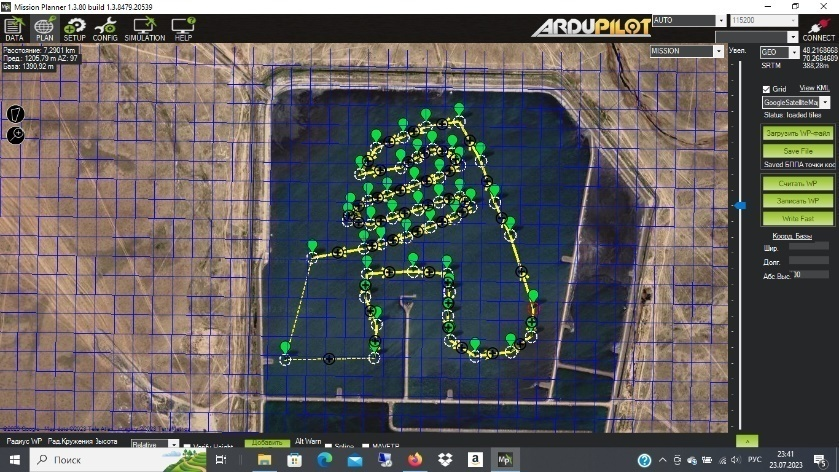
\includegraphics[width=0.7\textwidth]{assets/208}
	\caption*{\bfseries Рис. 1 -- Построение траектории в Mission Planner}
\end{figure}
\begin{multicols}{2}

Для анализа движения мобильных роботов проводились эксперименты с
использованием симуляторов и математических моделей релизованных на
Python, учитывающих влияние течения и других факторов. Полученные
результаты анализировались с целью определения оптимальных стратегий
управления в различных условиях.

Эксперименты включали в себя серию тестовых полетов и анализ движения
мобильных роботов в различных условиях. Перед началом экспериментов
проводилась подготовка оборудования и алгоритмов, а также калибровка
датчиков. Затем выполнялись запланированные полеты и сбор данных,
которые анализировались с использованием статистических и математических
методов. Полученные результаты использовались для оценки эффективности
разработанных методов и алгоритмов.

\emph{Навигационная система.} Для построения траектории с помощью HEX
Pixhawk 2.1 CUBE ORANGE+ необходимо использовать специализированные
программные пакеты и алгоритмы, позволяющие задать нужную траекторию
полета.

Это было реализовано с помощью программ-ного пакета Mission Planner. При
построении траектории с помощью HEX Pixhawk 2.1 CUBE ORANGE+ учитываются
различные параметры полета, такие как высота, скорость, курс и точки
назначения. Это позволяет управлять БППА в соответствии с заданными
целями и с высокой точностью выполнять требуемые маршруты \\(Рис. 1).

Важно отметить, что для успешного построения траектории и выполнения
автоном-ного полета с помощью HEX Pixhawk 2.1 CUBE ORANGE+ также
необходимо обеспечить правильную калибровку и настройку всех датчиков и
устройств, используемых на БППА. Кроме того, при использовании
беспилотных плавательных аппаратов критически важно обеспечение
безопасности полетов и соблюдение всех нормативных норм и правил (Рис.
2).

Для анализа движения мобильного робота представляется необходимым ввести
системы координат, описывающее его движения. При этом используются две
системы координат: фиксированная \(X_{0}OY_{0}\). и подвижная XGY,
жестко связанная со станком. Оси стационарной системы координат
выбираются в качестве начальных так, чтобы в начальный момент времени
они совпадали с осями движущейся системы.

Угол \(\lambda\), образующийся между диаметральной плоскостью (ДП) и
осью \(X_{0}\), называется курсовым углом. Этот угол можно выразить
через другие углы, например:

Центральный угол сноса (\(\varphi\)), который измеряется между вектором
мгновенной скорости центра тяжести (ЦТ) робота и диаметральной
плоскостью.
\end{multicols}

\begin{figure}[]
	\centering
	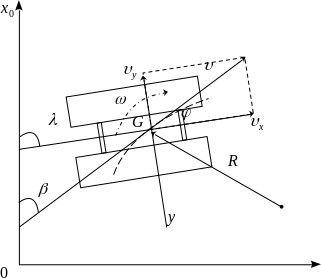
\includegraphics[width=0.5\textwidth]{assets/209}
	\caption*{\bfseries Рис. 2 -- Схема исследования траектории плавающего робота при
  повороте}
\end{figure}

\begin{multicols}{2}

Угол траектории (\(\beta\)) или угол скорости, который измеряется между
вектором скорости и \(X_{0}\) осью. Для оценки влияния течения на
управляемость плавающего робота анализируется их движение в двух
случаях: с течением и без течения. Это осуществляется путем построения
траекторий движения робота на основе исходных данных теста. Параметры
движения робота можно определить через проекцию скорости центра тяжести
на движущиеся оси и угловую скорость. Однако в некоторых ситуациях
удобнее использовать альтернативные кинематические параметры: модуль
скорости центра тяжести (│\(v\)│), угол сноса (\(\varphi\)) и угловую
скорость. Такая система параметров позволяет более удобно описывать
движение и анализировать его влияние на управляемость робота при
различных условиях течения {[}7{]}.

-- абсолютная скорость транспортного средства относительно системы
координат: угол траектории или угол скорости, измеренный между вектором
скорости и осью {[}8{]}.

v-- абсолютная скорость транспортного средства относительно системы
координат \(X_{0}OY_{0}\). : угол траектории или угол скорости,
измеренный между вектором скорости и осью \(X_{0}\) {[}7{]}.

\begin{equation}
  \begin{aligned}
  X &= \int_{0}^{t} v \cos(\beta) \, dt \\
  Y &= \int_{0}^{t} v \sin(\beta) \, dt
  \end{aligned}
  \end{equation}
  

В отсутствие потока (скорость потока равна нулю) траектория робота
подчиняется следующим принципам и уравнениям:
\end{multicols}

\begin{equation}
  \begin{aligned}
    X = \int_{0}^{t}v\cos(\beta + \omega t)dt = \int_{}^{}\left( v_{x} - at \right)\cos(\varphi + \omega t)dt \\
    Y = \int_{0}^{t}v\sin(\beta + \omega t)dt = \int_{}^{}\left( v_{y} - at \right)\sin(\varphi + \omega t)dt
  \end{aligned}
\end{equation}

\begin{multicols}{2}

Эти уравнения описывают прямолинейное равномерное движение робота без
учета влияния потока. Таким образом, при отсутствии потока машина будет
двигаться прямолинейно со скоростью \(v\) под углом к положительному
направлению оси X.

Траектория катамарана под действием течения определяется следующим
образом:
\end{multicols}

\begin{equation}
  \begin{aligned}
    X = \int_{}^{}v_{i}\cos(\beta + \omega t)dt = \int_{}^{}\left( \sqrt{v^{2} + v_{f}^{2} + v_{c}v_{t}\cos\left( \varphi_{f} \right)} \right)\cos(\beta + \omega t)dt \\
    Y = \int_{}^{}v_{i}\sin(\beta + \omega t)dt = \int_{}^{}\left( \sqrt{v^{2} + v_{f}^{2} + v_{c}v_{t}\sin\left( \varphi_{f} \right)} \right)\sin(\beta + \omega t)dt
  \end{aligned}
\end{equation}

\begin{multicols}{2}


При наличии течения абсолютная скорость \(v_{c}\) cотносительно системы
координат  \(X_{0}OY_{0}\) определяется, как показано на рисунке 3.

Результаты расчетной оценки влияния скорости течения на траекторию
движения катамарана с использованием программы Python.
\end{multicols}

\begin{figure}[H]
	\centering
	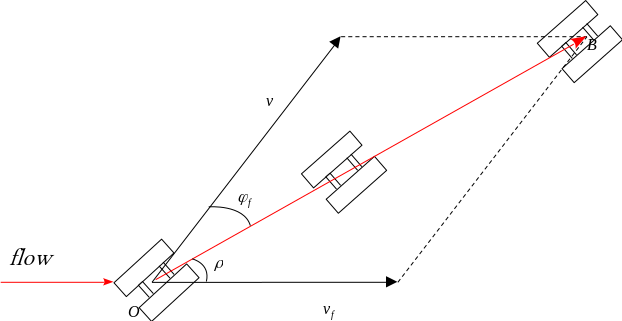
\includegraphics[width=0.6\textwidth]{assets/210}
	\caption*{\bfseries Рис. 3 -- Схема исследования траектории плавающего робота при повороте под действием потока воды}
\end{figure}



\begin{figure}[H]
	\centering
	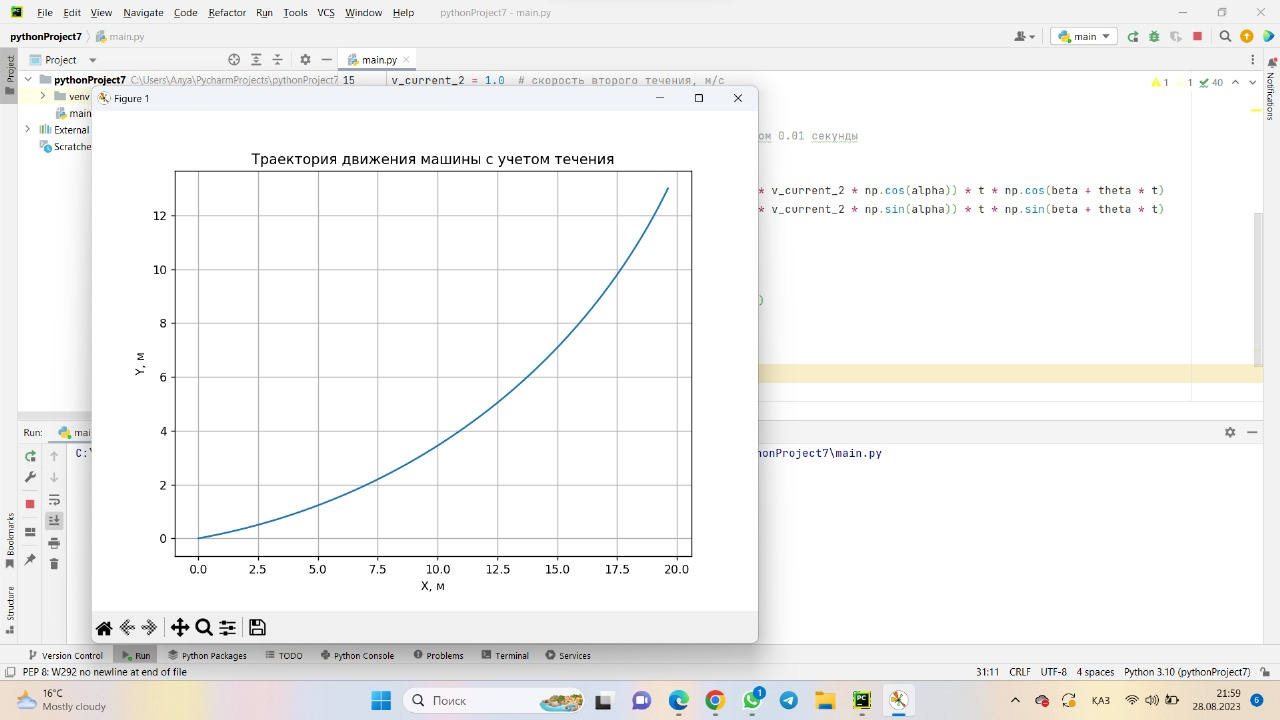
\includegraphics[width=0.3\textwidth]{assets/211}
	\caption*{\bfseries Рис. 4 -- Траектория катамарана в течение первых 10 секунд (без
  учета и без учета течения)}
\end{figure}


\begin{multicols}{2}

Для наглядности предположим, что мы хотим рассчитать траекторию
катамарана в течение первых 10 секунд (без учета и без учета течения)(Рис. 4).

Для расчета траектории катамарана с учетом скорости потока воды можно
модифицировать уравнения движения с учетом дополнительной скорости,
вызванной течением. Вам нужно будет сложить векторы скорости плавания и
вектор скорости потока, чтобы определить конечную скорость автомобиля:
По оси OX и OY. если масса машины 75 кг, длина 1,57 м, ширина 0,515 м,
высота 0,3, скорость плавания 0,5 м/с, угол сноса 0,1 рад., угол
скорости 0,2 рад., относительный радиус поворота 0,75 м., угол скорости
0,05 рад/с., скорость первого потока 1,4 м/с, скорость второго потока 1
м/с. Начальная координата 0,0.

\emph{Разработка программного обеспечения для получения 2D, 3D карт
дна.} Полученные данные с борта, в частности от эхолокационного
устройства (данные о глубине) и HEX Pixhawk 2.1 CUBE ORANGE+ (данные
GPS, данные о состоянии, данные о траектории), передаются в удаленный
командный центр (компьютер). Данные, полученные от HEX Pixhawk 2.1 CUBE
ORANGE+, отправляются в Mission Planner для мониторинга данных в
реальном времени, таких как координаты GPS, высота, скорость, состояние
батареи и другие параметры {[}9-10{]}. Эти данные можно сохранить в
текстовый файл и отправить на веб-сервер для последующего сохранения в
базе данных MySQL. Далее с помощью разработанного программного кода на
Python и его библиотек данные обрабатываются и визуализируются в 2D и 3D
графике. Для быстрой обработки используется библиотека Numpy,
позволяющая конвертировать данные в удобный для анализа массив.
Созданный таким образом массив визуализируется с помощью библиотеки
plotly. Для создания 2D и 3D графики используется экспресс-инструмент,
который, получая ранее созданный массив данных, создает динамическое
окно с графиками (Рис. 5). Затем Python создает html-файл с готовыми
графиками. В это окно добавлены CSS-классы для более удобного
интерфейса, с которым будет взаимодействовать пользователь (Рис. 6).
Готовый html-файл отправляется клиенту приложения, где пользователь
может его видеть и взаимодействовать с ним. На рисунке 5 3D карта дна
хвостохранилища Жайремского горно-обогатительного комбината. Объект был
исследован несколько раз для большей точности данных.
\end{multicols}
\begin{figure}[H]
	\centering
	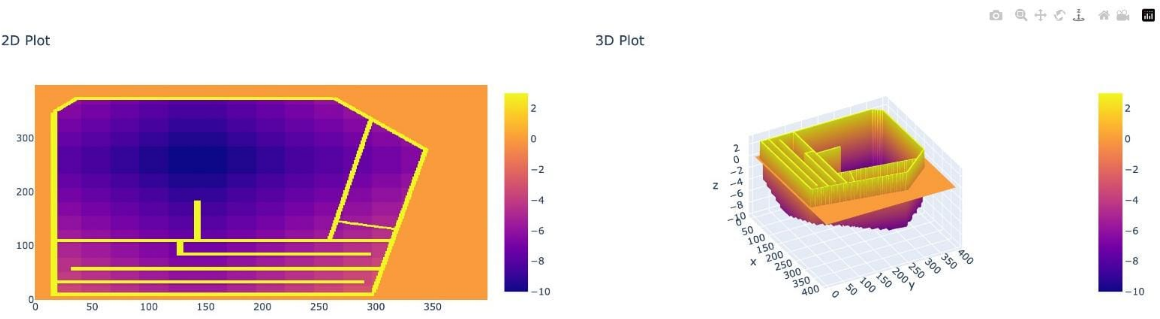
\includegraphics[height=0.3\textwidth, width=0.8\textwidth]{assets/212}
	\caption*{\bfseries Рис. 5 -- 2D, 3D карта дна хвостохранилища Жайремского
  горно-обогатительного комбината}
\end{figure}



\begin{figure}[H]
	\centering
	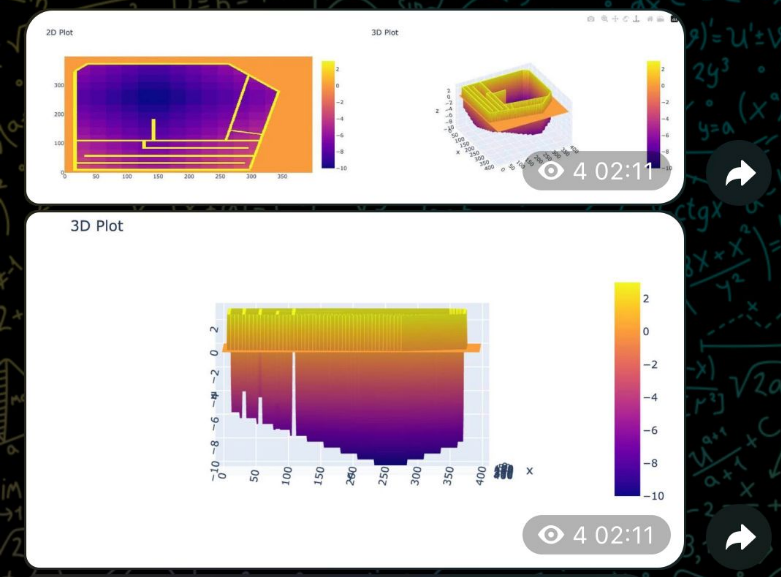
\includegraphics[width=0.5\textwidth]{assets/213}
	\caption*{\bfseries Рис. 6 -- Телеграм бот}
\end{figure}


\begin{multicols}{2}


По результатам испытаний робототехнического комплекса получены данные об
ошибке движения робота в системе координат, которая составляет примерно
0,2 метра по оси x и 0,1 метра по оси y. Во время испытаний температура,
влажность, уровень кислорода (O2) и концентрация частиц были практически
постоянными. Также известно, что средняя глубина хвостохранилища
составляет 4,56 метра.

На основании этих данных были произведены расчеты объема воды. Для этого
были замерены площади водосборов различных участков: площадь водосбора
участка баритового хвостохранилища - 2,5 км2, площадь водосбора участка
баритового хвостохранилища вместе с участком фильтрации - 0,38 км2.
Также установлено, что в пруду-окислителе скопилось 1,85 млн м3 воды,
что соответствует уровню воды на отметке 392,55 метра.

Результаты расчетов позволили установить следующие факты:

В первом полугодии 2021 года был «нулевой» баланс без сброса излишков в
пруд-испаритель. Этого удалось добиться за счет замачивания основания и
заполнения участков хвостохранилища, что предотвратило сброс воды.

За последующий период до конца 2023 года зафиксировано превышение
оборотной воды в пределах от 6704,443 до 24593,282 млн м3, которая
сбрасывалась в пруд-испаритель. Это позволило контролировать уровень
воды в системе и избежать перелива.

Также установлено, что площадь и объем прудов-отстойников участков
хвостохранилища и пруда-окислителя обеспечивают:

Достаточное освещение оборотной воды, возвращаемой на завод в
технологическом процессе, позволяет повторно использовать эту воду.

Возможность складирования объема хвостов, поступающих в пруды-отстойники
в течение года, что способствует эффективному обращению с отходами.

Натурные эксперименты, проведенные с использованием мобильного
роботизированного комплекса, позволили сделать вывод, что МРК
обеспечивает стабильную и надежную передачу данных. Преодоление помех,
возникающих на выходах датчиков, было достигнуто за счет внедрения схем
развязки, что значительно улучшило качество сигнала и обеспечило более
точные измерения. Программное обеспечение, предназначенное для
эффективного контроля и мониторинга функций работы системы при
использовании на персональном ноутбуке. Это обеспечивает полный спектр
функциональных возможностей предлагаемой системы и обеспечивает ее
высокую практичность в реальных условиях эксплуатации. Следует отметить,
что внедрение датчика воды в БППА дает водникам уникальную возможность
осуществлять непрерывный мониторинг и контроль параметров качества воды
на уязвимых и стратегически важных участках хвостохранилищ и водоемов.
Такой подход значительно повышает эффективность и результативность
управления водными ресурсами, способствуя более рациональному и
обоснованному принятию решений в этой области.

{\bfseries Результаты и обсуждение.} Рисунок 1 демонстрирует графическое
представление траекторий полета БППА для разных сценариев. На рисунке 5
представлена 3D карта дна хвостохранилища Жайремского
горно-обогатительного комбината, которая была визуализирована в
результате ряда экспериментов с применением разработанного
исследовательской группой проекта AP09058557 и авторами статьи МРК, над
хвостохранилищем. Объект был исследован несколько раз для большей
точности данных.

Исследование направлено на разработку и апробацию методов планирования
траекторий для БППА с использованием программного пакета Mission
Planner. Основной целью было улучшение точности и эффективности
управления беспилотными аппаратами.

Наиболее значимые результаты включают улучшение времени полета и
точности навигации при использовании новых алгоритмов планирования
траекторий. Сравнение с другими исследованиями показывает сопоставимые
или более высокие показатели эффективности разработанных методов. Однако
проблемные зоны включают необходимость дальнейшей оптимизации алгоритмов
для учета разнообразных условий полета.

В данной работе был представлен процесс построения траектории полета для
беспилотных аппаратов с использованием HEX Pixhawk 2.1 CUBE ORANGE+ и
программного пакета Mission Planner. Этот процесс включает в себя учет
различных параметров полета, таких как высота, скорость и курс, и
позволяет эффективно управлять беспилотными аппаратами в соответствии с
заданными целями. Основное внимание уделено безопасности и настройке
датчиков и устройств, необходимых для автономного полета. Проведенный
анализ движения мобильного робота, включая оценку углового ускорения и
скорости с учетом воздействия течения, позволяет более точно планировать
маршруты и управлять беспилотными аппаратами в различных условиях.
Дополнительно, рассмотрены методы разработки программного обеспечения
для получения и обработки данных о глубине морского дна с использованием
HEX Pixhawk 2.1 CUBE ORANGE+ и эхолокационного устройства. Этот подход
открывает новые перспективы для исследования морских ресурсов с высокой
точностью и безопасностью. Таким образом, представленная методика и
результаты работы имеют важное значение для разработки и управления
беспилотными аппаратами, а также для проведения исследований морского
дна и его ресурсов. Дальнейшие исследования в этой области могут
включать расширение функциональности программного обеспечения, а также
углубленный анализ влияния различных параметров на эффективность
управления беспилотными аппаратами.

{\bfseries Выводы\emph{.}} В ходе исследования были рассмотрены методы
планирования траекторий для беспилотных аппаратов с использованием
программного пакета Mission Planner. Полученные результаты позволяют
сделать вывод о повышении точности и эффективности управления БППА в
различных сценариях полета. Были изучены специализированные программные
пакеты и алгоритмы для планирования траекторий полета беспилотных
аппаратов. Разработаны и апробированы методы построения траекторий с
использованием оборудования HEX Pixhawk 2.1 CUBE ORANGE+ и программного
пакета Mission Planner. Проведен анализ движения мобильных роботов с
учетом воздействия течения, что позволило определить оптимальные
стратегии управления в различных условиях. Полученные результаты
подтверждают гипотезу о том, что применение специализированных методов
планирования траекторий повышает эффективность управления беспилотными
аппаратами. Таким образом, разработанные методы и алгоритмы имеют
потенциал для широкого применения в области автономных систем и могут
быть использованы для улучшения точности и эффективности управления
беспилотными аппаратами.

\emph{{\bfseries Финансирование.} Работа выполнена при поддержке гранта МОН
РК в рамках проекта AP09058557 по договору No63-КМУ2 от 24 февраля 2021
года.}
\end{multicols}

\begin{center}
  {\bfseries Литература}
  \end{center}

\begin{noparindent}

\begin{enumerate}
\def\labelenumi{\arabic{enumi}.}
\item
  Shubhani Aggarwal, Neeraj~Kumar. Path planning techniques for unmanned
  aerial vehicles: A review, solutions, and challenges // Computer
  Communications. - 2020. -- Vol. 149. - P. 270-299. DOI:
  10.1016/j.\\comcom.2019.10.014.
\item
  Faiyaz Ahmed, J.C. Mohanta, Mohd. Nayab Zafar. Development of smart
  quadcopter for autonomous overhead power transmission line inspections
  // -- 2022. -- Vol. 51(1). -P. 261-268. DOI:
  10.1016/j.matpr.\\2021.05.271
\item
  How to connect a PixHawk Cube or similar system - a simple overview.
  --URL: https://www.youtube.com/\\watch?v=tIE8IN71UFI. (date of
  application15.06.2024)
\item
  All the confusing names in \textquotesingle Pixhawk\textquotesingle{}
  explained (Mission Planner, PX4, Ardupilot Pixhawk etc.) --\\URL:
  https://www.youtube.com/watch?v=0vBXFjhw-5M. (date of
  application15.06.2024)
\item
  Khosyi\textquotesingle In, M., Budisusila, E.N., Dwi Prasetyowati
  S.A., Suprapto B.Y.; Nawawi Z. Design of Autonomous Vehicle Navigation
  Using GNSS Based on Pixhawk 2.1 // International Conference on
  Electrical \\Engineering, Computer Science and Informatics
  (EECSI)\emph{.} -- 2021. -P. 175 -- 180. DOI:
  10.23919/EECSI\\53397.2021.9624244.
\item
  Mission Planner Overview, 2021, {[}online{]} Available. --URL:
  htt://ardupilot.org/planner/docs/mission-planner-overview.html. (date
  of application15.06.2024)
\item
  Myasischev, O. O., Lienkov, S. V., Ovcharuk, V. V., Tolok, I.,
  Lytvynenko, N., Zinchyk, A. G., \& Lytvynenko, O. I. Large-capacity
  quadcopter's designing on the controllers of the pixhawk cube family.
  75. -2022. --P. 108-118. DOI: 10.17721/2519-481x/2022/75-11
\item
  S. Fujita and S. Mae Causes and Nature of ice-sheet radio-echo
  internal reflection estimated from the dielectric properties of ice //
  Annals of glaciology. -1994. -Vol. 20. -P. 80-86.
\item
  Nicolas A.; Olmedo and Michael G. Lipsett. 2016. Design and field
  experimentation of a robotic system for tailings characterization //
  Journal of Unmanned Vehicle Systems. --Vol. 4(3). --P. 169-192. DOI
  10.1139/juvs-2015-0034.
\item
  Lienkov, S., Myasischev, A. A., Ovcharuk, V., Lenkov, E., \&
  Lytvynenko, N.. Development of \\Multifunctional Rotary UAV Based on
  Pixhawk Family Flight Controllers. -2023. --Vol. 18(1). DOI:
  10.3849/aimt.01752
\end{enumerate}
\end{noparindent}

\emph{{\bfseries Сведения об авторах}}
\begin{noparindent}

Жартыбаева М.Г.-PhD., Евразийский национальный университет им. Л. Н.
Гумилева, Астана,\\Казахстан, e-mail: makkenskii@mail.ru;

Алинова А.Д.-Евразийский национальный университет им. Л. Н. Гумилева,
Астана, Казахстан,\\ e-mail: alinova-aida@mail.ru;

Оралбекова Ж.О. -PhD, Евразийский национальный университет имени Л.Н.
Гумилева, Астана, \\Казахстан, e-mail: oralbekova@bk.ru;

Тюлепбердинова Г.А.-к.ф.-м.н., доцент, Казахский национальный
университет им. Аль-Фараби,\\ Алматы, Казахстан, e-mail:
tyulepberdinova@gmail.com;

Жамишева Н.М.-\/-«Институт законодательства и правовой информации
Республики Казахстан»\\ Министерства юстиции Республики Казахстан, главный
специалист отдела поддержки информаци-онных систем, Астана, Казахстан,
e-mail: nuray\_zhamisheva33@gmail.com.
\end{noparindent}

\emph{{\bfseries Information about the authors}}
\begin{noparindent}

Zhartybayeva M.G. -PhD., L. N. Gumilyov Eurasian National University,
Astana, Kazakhstan, \\e-mail: makkenskii@mail.ru;

Alinova A/D.- L. N. Gumilyov Eurasian National University, Astana,
Kazakhstan, \\e-mail: alinova-aida@mail.ru;

Oralbekova Zh. O. -Ph.D., L.N. Gumilyov Eurasian national university,
Astana, Kazakhstan, \\e-mail: oralbekova@bk.ru;

Tyulepberdinova G.A.- PhD, associate professor, Al-Farabi Kazakh
National University, Almaty, \\Kazakhstan, e-mail:
tyulepberdinova@gmail.com;

Zhamisheva N.M. - Institute of Legislation and Legal information of the
Republic of Kazakhstan" Ministry of Justice of the Republic of
Kazakhstan, Chief specialist of the information systems support
department, Astana, Kazakhstan, e-mail: nuray\_zhamisheva33@gmail.com.


\end{noparindent}


